\documentclass[../../main.tex]{subfiles}
\begin{document}

\chapter{CostCompiler}
CostCompiler è un interprete per il linguaggio di programmazione definito nel capitolo precedente Grammatica \ref{sec:grammatica}. Una volta ricevuto il programma, CostCompiler procede alla verifica e correttezza sintattica e semantica del programma, successivamente si occupa della generazione dell'albero di sintassi astratta. 
Questo albero rappresenta una versione astratta del programma, che astrae i dettagli sintattici del codice e si concentra sulla sua struttura logica, associando ad ogni costrutto (eg.\textit{if-then-else} un unico nodo, \textit{IfNode} presente nel omonimo file in src/ast) i rispettivi sottonodi(nel caso di \textit{IfNode} conterrà la guardia condizionale e i due statement).
Dopo aver generato l'albero di sintassi astratta, CostCompiler si occupa della verifica Semantica \ref{sec:semantica} del linguaggio andando ad effettuare i controlli semantici e di tipo sul programma in input, andando a garantire alcune invarianti (eg. le chiamate di funzioni devono rispettare i tipi di ritorno).\\
Una volta effettuata la verifica semantica, CostCompiler procede con la generazione delle equazioni di costo, andando a visitare l'AST secondo determinati criteri, ad ogni nodo figlio verrà passata una Mappa che contiene la mappatura di ogni variabile in una stringa che sarà la stessa stringa che compare nelle equazioni di costo.\\
Ogni nodo figlio invocato attraverso la funzione \textit{toEquation()} ritorna una stringa, rappresentante l'equazione di costo del nodo figlio, e il padre va a concatenare le stringhe dei figli(anche in base al tipo di figlio da cui ricevere l'equazione), ad esempio la \textit{return $<$EXP$>$ } sarà diverso dal \textit{return }$<$function$(Par)>$.\\
Il risultato finale di questo processo di concatenazione attraverso determinati nodi dell'AST è la generazione delle equazioni di costo. 
Una volta generate le equazioni di costo, CostCompiler le stampa in un file \textit{equation.ces}, inoltre lancia il risolutore PUBS \ref{sec:pubs} che va a calcolare gli upper bound del programma da stampare a video.
Riportiamo un esempio di equazione di costo generata da CostCompiler dato un programma scritto in HLCostLang:
    \begin{lstlisting}[language=Java, caption={Listing8}]
    struct Params {
        address: array[int],
        payload: any,
        sender: string
    }
    service PremiumService : (string) -> void;
    service BasicService : (any) -> void;
    (isPremiumUser: bool, par: any) => {
        if ( isPremiumUser ) {
            call PremiumService("test");
        } else {
            call BasicService( par);
        }
    }
\end{lstlisting}
Una volta preso in input Listing8, CostCompiler genera le seguenti equazioni di costo:
\begin{lstlisting}[language=Java, caption={Equazioni di costo per Listing8}]
eq(main(P,ISPREMIUMUSER0,B),0,[if9(ISPREMIUMUSER0,P,B)],[]).
eq(if9(ISPREMIUMUSER0,P,B),nat(P),[],[ISPREMIUMUSER0=1]).
eq(if9(ISPREMIUMUSER0,P,B),nat(B),[],[ISPREMIUMUSER0=0]).
\end{lstlisting}
Andando a descriverle ci troveremo ad avere una equazione per la regola \textit{init}, dove vediamo che \textit{main} viene chiamata con costo 0 e verrà chiamata \textit{if9} con parametri \textit{ISPREMIUMUSER0,P,B}.\\
$P$ e $B$ sono il costo costante delle chiamate ai servizi \textit{isPremiumUser} e \textit{BasicService}, mentre \textit{ISPREMIUMUSER0} sarà la valutazione del parametro \textit{isPremiumUser} che sarà 1 se vero, 0 altrimenti; in altri termini \textit{ISPREMIUMUSER0} sarà la valutazione della guardia del costrutto \textit{if-then-else} e verrà eseguita la chiamata al servizio \textit{PremiumService} se \textit{ISPREMIUMUSER0} sarà 1 con costo $nat(P)$, altrimenti verrà eseguita la chiamata al servizio \textit{BasicService} con costo $nat(B)$. 
Una volta avere generato l'equazioni di costo dal programma, lo stampiamo in un file \textit{equation.ces}, cosi da poter eseguire PUBS(A Practical Upper Bounds Solver), per determinarci l'Upper Bound del programma.
L'obiettivo di PUBS(come vedremo in seguito \ref{sec:pubs}) è quello di ottenere automaticamente upper bound in forma chiusa per i sistemi di equazioni di costo, di conseguenza calcola i limiti superiori per la relazione di costo indicata come "Entry", oltre che per tutte le altre relazioni di costo di cui tale "Entry" dipende.
\section{Implementazione}

Il codice è strutturato in modo gerarchico, partendo dall'interfaccia \textit{Node}, che viene estesa dai nodi che compongono l'AST e che contiene la firma dei metodi che ogni nodo deve implementare.\\

\begin{lstlisting}[language=Java, caption={Interfaccia Node}]
package ast;

public interface Node {
    EnvVar checkVarEQ(EnvVar e);
    Node typeCheck(Environment e) throws TypeErrorException;
    ArrayList<String> checkSemantics(Environment env);
    String toEquation(EnvVar e);
    String codeGeneration(HashMap<Node, Integer> offset_idx);
}

\end{lstlisting}
Andando a descrivere i metodi dell'interfaccia Node:
\begin{itemize}
    \item \textit{checkVarEQ(EnvVar e)}: Questo metodo prende in input un oggetto di tipo \textit{EnvVar} che è un HashMap che mappa un oggetto di tipo \textit{Node} con una stringa, che rappresenta la variabile che mappa quel determinato nodo. Questo metodo ritorna un oggetto di tipo \textit{EnvVar} che rappresenta l'ambiente aggiornato con le variabili mappate con le stringhe corrispondenti.
    \item \textit{typeCheck(Environment e)}: Questo metodo prende in input un oggetto di tipo \textit{Environment} che rappresenta l'ambiente in cui si trova il nodo, e ritorna un oggetto di tipo \textit{Node} che rappresenta il nodo tipato, dopo aver effettuato il controllo di tipo.
    \item  \textit{checkSemantics(Environment env)}: Questo metodo prende in input un oggetto di tipo \textit{Environment} e rappresenta il controllo semantico del nodo, ritorna un oggetto di tipo \textit{ArrayList$<$String$>$} che rappresenta una lista di stringhe che rappresentano eventuali errori semantici.
    \item \textit{toEquation(EnvVar e)}: Questo metodo prende in input un oggetto di tipo \textit{EnvVar}, che mappa determinati nodi secondo quell'oggetto, e rappresenta la generazione delle equazioni di costo del nodo, ritorna un oggetto di tipo \textit{String} che rappresenta l'equazione di costo del nodo.
    \item \textit{codeGeneration()}: Prende in input un oggetto di tipo \textit{HashMap$<$Node, Integer$>$} che mappa un nodo con un intero, utilizzato per le strutture dati complesse. \textit{offset\_idx} contiene l'indice delle strutture dati complesse rispetto alla memoria lineare. Inoltre il metodo \textit{codeGeneration} ritorna un oggetto di tipo \textit{String} che rappresenta il codice generato del nodo.
\end{itemize}
Ogni nodo dell'AST estende l'interfaccia \textit{Node} e implementa i metodi definiti in essa. 
Dopo aver definito l'interfaccia \textit{Node}, andiamo a definire le fasi di sviluppo del nostro AST.
In prima fase grazie al plugin ANTLR, dopo aver definito il file \textit{HLCostLang.g4} che rappresenta la grammatica del nostro linguaggio, ANTLR ci genera i file \textit{HLCostLangLexer.java} e \textit{HLCostLangParser.java} che rappresentano rispettivamente il Lexer e il Parser del nostro linguaggio. 
L'interfaccia \textit{HLCostLangVisitor.java} e \textit{HLCostLanListener.java} vengono generate da ANTLR e rappresentano rispettivamente le interfacce per la generazione di un albero di parsing. 
Tutti i file generati automaticamente da ANTLR li troviamo nella cartella \textit{src/gen}.
All'interno di questa cartella troviamo anche il file \textit{HLCostLangBaseVisitor.java} che rappresenta la classe base per la generazione dell'AST, che andiamo a implementare per generare il nostro albero di parsing nel file \textit{HLCostLangBaseVisitorImpl.java}.\\
\begin{lstlisting}[language=Java, caption={Implementazione del Visitor AST}] 
public class HLCostLanBaseVisitorImpl extends          HLCostLanBaseVisitor<Node> {
@Override
public Node visitPrg(PrgContext ctx) {
    ArrayList<Node> complexType = new ArrayList<>();
    ArrayList<Node> decServices = new ArrayList<>();
    ArrayList<Node> funDec = new ArrayList<>();

    for (ServiceDeclContext decService : ctx.serviceDecl()){
        decServices.add(visitServiceDecl(decService));
    }

    for (FunctionDeclContext fund : ctx.functionDecl()) {
        funDec.add(visitFunctionDecl(fund));
    }

    for(ComplexTypeContext complexTypeContext : ctx.complexType()){
        complexType.add(visitComplexType(complexTypeContext));
    }
    return new ProgramNode(complexType, decServices, funDec, visitInit(ctx.init()));
}

    ...
\end{lstlisting}
Qui vediamo l'implementazione del metodo \textit{visitPrg} che rappresenta la creazione del nodo \textit{ProgramNode} che rappresenta il nodo principale del nostro AST.\\
Come vediamo il metodo \textit{visitPrg} prende in input un oggetto di tipo \textit{PrgContext} che rappresenta il contesto riconosciuto rispetto alla grammatica di riferimento, e ritorna un oggetto di tipo \textit{Node} che rappresenta il nodo principale del nostro AST.\\
Come vediamo \textit{complexType, decServices, funDec} sono rispettivamente le liste di nodi che rappresentano i tipi complessi, le dichiarazioni dei servizi e le dichiarazioni delle funzioni, sono definiti come Arraylist$<$Node$>$, perchè andremo ad iterare sui contesti specificati per fare in modo che ogni contesto venga visitato e ritorni un oggetto di tipo \textit{Node} che rappresenta il nodo del nostro AST.\\
Una volta visitati tutti i contesti, andiamo a creare il nodo \textit{ProgramNode} che rappresenta il nodo principale del nostro AST, che conterrà la lista dei nodi dei tipi complessi, delle dichiarazioni dei servizi e delle dichiarazioni delle funzioni, e la chiamata iniziale \textit{init}.\\
Una volta generato il nodo principale del nostro AST, andiamo a visitare tutti i nodi figli ricorsivamente, andando a creare i rispettivi nodi del nostro AST, che rappresentano il programma in input.\\

\subsubsection{Controllo Semantico}
Il controllo semantico è un processo che verifica la correttezza semantica del programma, ovvero verifica che il programma sia corretto rispetto alle regole del linguaggio.\\
Il controllo semantico viene effettuato attraverso il metodo \textit{checkSemantics(Environment env)} che prende in input un oggetto di tipo \textit{Environment} e ritorna un oggetto di tipo \textit{ArrayList$<$String$>$} che rappresenta una lista di stringhe che rappresentano eventuali errori semantici.\\
Il controllo semantico viene effettuato in modo ricorsivo, partendo dal nodo principale del nostro AST, andando a visitare tutti i nodi figli, e andando a verificare che il programma sia corretto rispetto alle regole del linguaggio.\\
Il controllo semantico viene specificato nel \textit{main.java} presente all'interno della cartella \textit{src/com/company} e rappresenta il punto di partenza del nostro programma.
\newpage
\begin{lstlisting}[language=Java, caption={Inizio Controllo semantico }]
    HLCostLanBaseVisitorImpl visitor = new HLCostLanBaseVisitorImpl();
    Node ast = visitor.visit(parser.prg());
    Environment env = new Environment();
    ArrayList<String> errorSemantics = ast.checkSemantics(env);
    if (!errorSemantics.isEmpty()) {
        System.err.println(errorSemantics);
        return Results.SEMANTIC_ERROR;
    }else{
        //continua l'esecuzione del programma
    }
\end{lstlisting}
Come vediamo, viene istanziato un visitor di tipo \textit{HLCostLanBaseVisitorImpl} che rappresenta il visitor del nostro AST, e viene visitato il contesto \textit{prg()} che rappresenta il contesto principale del nostro programma.\\
Una volta visitato il contesto, andiamo a creare l'ambiente \textit{env} che rappresenta l'ambiente in cui si trova il nostro programma, andiamo a chiamare il metodo \textit{checkSemantics(Environment env)} che rappresenta il controllo semantico del nostro programma, e ritorna una lista di stringhe che rappresentano eventuali errori semantici. Per controllare che il programma sia corretto rispetto alle regole del linguaggio basta controllare che la lista ritornata sia vuota, in caso contrario stampiamo gli errori semantici e terminiamo l'esecuzione del programma.\\

\begin{lstlisting}[language=Java, caption={Controllo semantico di ForNode}]
@Override
public ArrayList<String> checkSemantics(Environment env) {
    ArrayList<String> errors = new ArrayList<>();
    if(!env.checkHeadDeclaration(id))
        env.addDeclaration(id,new IntType());
    else
        errors.add("Error: Variable "+id+" already declared");

    errors.addAll(exp.checkSemantics(env));
    errors.addAll(stm.checkSemantics(env));
    return errors;
}
\end{lstlisting}
Come vediamo, il metodo \textit{checkSemantics(Environment env)} prende in input un oggetto di tipo \textit{Environment} e ritorna un oggetto di tipo \textit{ArrayList$<$String$>$} che rappresenta una lista di stringhe che rappresentano eventuali errori semantici.
Il metodo \textit{checkSemantics(Environment env)} viene implementato in modo ricorsivo, partendo dal nodo principale del nostro AST, andando a visitare tutti i nodi figli, e andando a verificare che il programma sia corretto rispetto alle regole del linguaggio.
Come vediamo nel \textit{ForNode} andiamo a verificare che la variabile \textit{id} sia dichiarata all'interno dell'ambiente \textit{env}, e in caso contrario la aggiungiamo all'ambiente, altrimenti andiamo a stampare un errore semantico, e successivamente andiamo a visitare i nodi figli \textit{exp} e \textit{stm} e andiamo a concatenare gli errori semantici ritornati dai nodi figli.
\subsubsection{Controllo dei tipi}
Il controllo dei tipi è un processo che verifica che il programma sia corretto rispetto ai tipi del linguaggio, ovvero verifica che le espressioni siano corrette rispetto ai tipi del linguaggio.
Il controllo dei tipi viene effettuato attraverso il metodo \textit{typeCheck(Environment e)} che prende in input un oggetto di tipo \textit{Environment} e ritorna un oggetto di tipo \textit{Node} che rappresenta il nodo tipato, dopo aver effettuato il controllo di tipo, inoltre il metodo \textit{typeCheck(Environment e)} può lanciare un'eccezione di tipo \textit{TypeErrorException} in caso di errore di tipo, che in caso viene catturata dal main e stampata a video.\\
Osserviamo un esempio di controllo di tipo:
\begin{lstlisting}[language=Java, caption={Controllo di tipo di CallNode}]
public Node typeCheck(Environment e) throws TypeErrorException {
    try {
        FunDeclarationNode fun = (FunDeclarationNode) e.getDeclaration(id.getId());
        FormalParams fp = fun.getFormalParams();
        if (fp.size() != listCount.size()) {
            throw new TypeErrorException("Wrong number of parameters in call " + id.getId());
        }
        for (int i = 0; i < listCount.size(); i++) {
            if (!Utils.isSubtype(fp.get(i).b.typeCheck(e), listCount.get(i).typeCheck(e))) {
                throw new TypeErrorException("Incompatible type in call node");
            }
        }
        return fun.getReturnNode().typeCheck(e);
    }catch (ClassCastException ex){
        throw new TypeErrorException("Error in call node");
    }
}
\end{lstlisting}
Come vediamo, il metodo \textit{typeCheck(Environment e)} prende in input un oggetto di tipo \textit{Environment}, da li controlla che la funzione chiamata (sappiamo che è gia definita perché prima effettuiamo il controllo semantico) abbia lo stesso numero di parametri che stiamo passando, e che i tipi dei parametri siano compatibili con i tipi dei parametri della funzione chiamata.
Viene inoltre, ritornato il tipo di ritorno della funzione chiamata.\\
Il metodo \textit{Utils.isSubtype(fp.get(i).b.typeCheck(e), listCount.get(i).typeCheck(e))} è un metodo di utilità che controlla se il tipo del parametro passato è sottotipo del tipo del parametro della funzione chiamata.\\
Qui di seguito invece osserviamo la dichiarazione del metodo \textit{isSubtype}:
\begin{lstlisting}[language=Java, caption={Metodo isSubtype}]
    public static boolean isSubtype(Node a, Node b) {
        return a.getClass().isAssignableFrom(b.getClass()); 
    }
\end{lstlisting}
Ritorna true se il tipo di \textit{a} è sottotipo del tipo di \textit{b}, altrimenti false.\\
Questo è possibile grazie al fatto che ogni nodo di tipo, viene esteso da uno specifico nodo supertipo. In questo caso abbiamo deciso che il tipo \textit{AnyType} estende il tipo \textit{IntType}, e tutti gli altri sottonodi che implementano l'interfaccia \textit{NodeType}, che rappresenta il tipo di un nodo.\\

In seguito verrà specificato come vengono generati le equazioni di costo\ref{sec:costEquation} attraverso il metodo \textit{toEquation(EnvVar e)} e come viene generato il WASM corrispondente andando a visitare l'AST con il metodo \textit{codeGeneration}\ref{sec:codeGeneration}.\\ 
\subsection{Struttura del codice}
Andiamo ad illustrare ora come abbiamo strutturato il codice, all'interno di \textit{src} troviamo le seguenti cartelle:
\begin{itemize}
    \item \textit{ast}: Contiene tutti i nodi che compongono l'AST, ogni nodo estende l'interfaccia \textit{Node} e implementa i metodi definiti in essa.
    \item \textit{com/company}: Contiene il file \textit{main.java} che rappresenta il punto di partenza del nostro programma, e contiene la logica principale del nostro programma.
    \item \textit{gen}: Contiene i file generati automaticamente da ANTLR, che rappresentano il Lexer e il Parser del nostro linguaggio, e le interfacce per la generazione dell'AST.
    \item \textit{utilities}: Contiene i file di utilità, come \textit{Environment.java}, \textit{TypeErrorException.java} che rappresenta l'eccezione lanciata in caso di errore di tipo, \textit{Utils.java} che contiene metodi di utilità generica.
    \item \textit{test}: Contiene i file di test, che descrivono i test del nostro programma, su un sottoinsieme di programmi scritti in HLCostLang.
\end{itemize}
All'interno di \textit{ast} troviamo tutti nodi che compongono l'ast suddivisi in base al tipo di nodo, ad esempio \textit{CallNode.java} che rappresenta il nodo di una chiamata a funzione, \textit{IfNode.java} che rappresenta il nodo di un costrutto \textit{if-then-else} si trovano all'interno della cartella \textit{ast/stm}.
Nodi come \textit{BinExpNode.java} che rappresenta il nodo di un'espressione binaria, \textit{DerExpNode.java} che rappresenta un identificativo, si trovano all'interno della cartella \textit{ast/exp}.
Nodi che servono per il controllo dei tipi come \textit{IntType.java} che rappresenta il tipo intero, \textit{BoolType.java} che rappresenta il tipo booleano, si trovano all'interno della cartella \textit{ast/typeNode}.
La cartella \textit{utilities} contiene i file di utilità, come \textit{Environment.java} che rappresenta l'ambiente in cui si trova il nostro programma, \textit{TypeErrorException.java} che rappresenta l'eccezione lanciata in caso di errore di tipo, \textit{Utils.java} che contiene metodi di utilità come \textit{isSubtype}.\\
La cartella \textit{test} contiene i file di test, che rappresentano i test del nostro programma, su un sottoinsieme di programmi scritti in HLCostLang.\\
I test sono stati scritti in modo da testare il corretto funzionamento del nostro programma, e sono stati scritti in modo da testare il corretto funzionamento del controllo semantico, del controllo dei tipi, della generazione delle equazioni di costo e del codice WASM corrispondente.\\
Il test ritorna un enumerato con il codice di errore specificato, in caso di errore, altrimenti ritorna \textit{Results.PASS}.
Alla fine di ogni sviluppo di una nuova funzionalità, andiamo a testare il corretto funzionamento del nostro programma, andando a eseguire i test, e verificando che il programma sia corretto rispetto alle regole del linguaggio.\\
\begin{lstlisting}[language=Java, caption={Esempio Testing}]
public class TestCostCompiler {

    @Test
    public void test1() throws IOException {
            System.out.println("Test Listing 1");
            assertEquals(CostCompiler("example/Listing1"), Results.PASS);
        }
    ...
\end{lstlisting} 
Il test è molto semplice, prende in input un programma in HLCostLang e verifica che la compilazione termini correttamente, in caso contrario stampa un errore a video, questo è un esempio banale di testing, ma ci permette di verificare che il programma sia corretto rispetto alle regole del linguaggio.\\
Inoltre ci sono altri test che verificano che il programmi ritorni degli errori specifici, definiti in base al tipo di errore, ad esempio se il programma non termina correttamente, se il programma ritorna un errore semantico, se il programma ritorna un errore di tipo, oppure se il programma ritorna un errore di compilazione, e cosí via.\\

\section{Regole di Inferenza}
\label{sec:inference_rule}
I programmi di costo sono elenchi di equazioni che hanno termini:
$$f(\overline{x} ) = e + \sum_{i \in 0..n} f_i (\overline{e_i}) \quad \quad \quad \quad[\varphi ]$$
Dove le variabili si presentano nel lato destro e in $\varphi $ sono un sottoinsieme di $\overline{x}$; mentre $f$ e $f_i$ sono i simboli delle funzioni.
Ogni funzione ha un right-hand-side che è un'espressione aritmetica che può contenere:
\begin{itemize}
    \item Un'espressione in Presburger aritmetica (PA)\autocite{DBLP:journals/corr/Haase14}:
    $$e ::= x \quad | \quad q \quad | \quad e + e \quad | \quad e - e \quad | \quad q \cdot e \quad |  max(e_1,\dots,e_n)$$
    Dove $x$ è una variabile, $q$ è una costante intera, $e_1,\dots,e_n$ sono espressioni aritmetiche e $max$ è un operatore che restituisce il massimo valore tra le sue espressioni.
    \item Un numero di invocazioni di funzioni di costo: $f_i (\overline{e_i})$.
    \item La guardia $\varphi$ è un vincolo congiuntivo lineare nella forma: $e_1 \geq e_2$ dove $e_1$ e $e_2$ sono espressioni aritmetiche di Presburger.
\end{itemize} 

La soluzione di un equazione di costo è il calcolo dei limiti di un particolare simbolo di una funziona(generalmente la prima equazione) e i limiti sono parametrici nei parametri formali dei simboli della funzione.
Definiamo un insieme di regole di inferenza che raccolgano frammenti di programmi di costo che vengono poi combinati in modo diretto dalla sintassi.
Usiamo una variabile di ambiente $ \varGamma $ come dizionari:
\begin{itemize}
    \item $\varGamma$ prende un servizio o un parametro e ritorna un espressione aritmetica di Presburger che di solito è una variabile.
    \item Quando scriviamo $\varGamma + i : \quad Nat $, assumiamo che i non appartenga al dominio di $\varGamma$.
\end{itemize}
I giudizi hanno forma:
\begin{itemize}
    \item $\varGamma \vdash E: e$, che significa che il valore dell'espressione intera E in $\varGamma$ è rappresentato (dall'espressione nell'aritmetica di Presburger) $e$
    \item $\varGamma \vdash E : \varphi$, significa che l'espressione booleana E in $\varGamma$ è rappresentata da $\varphi$
    \item $\varGamma \vdash S : e ; C; Q $, significa che il costo di S nell'ambiente $\varGamma$ è $e + C$ dato un insieme di equazioni Q
    \item $\varGamma \vdash F : Q$, significa che il costo di F nell'ambiente $\varGamma$ è rappresentato da un insieme di equazioni Q
\end{itemize}


\begin{align}
    &\mathrule{main}{
        \begin{aligned} \varGamma \vdash S : e ; C; Q  \quad \quad
        \overline{w} = \text{Var}(\overline{p},e) \cup \text{Var(C)}
        \end{aligned}
        }{\varGamma \vdash \overline{p}  \rightarrow \{S\}: 0 ;\emptyset;Q';C} \\
    &\mathrule{call}{\varGamma \vdash S : e ; C; Q}{\varGamma \vdash \text{call h}(\overline{E}) S : e + e' ; C; Q}\\
    &\mathrule{if}{
    \begin{aligned}
        &\varGamma \vdash E : \varphi  \quad \quad \varGamma \vdash S : e'; C; Q \quad \varGamma \vdash S : e"; C'; Q'\\
        &W = Var(e, e', e") \cup Var(C) \quad \quad \quad Q" =\big[ \begin{aligned}
            &\text{if}_l(\overline{w})  = e'+c[\varphi]\\
            &\text{if}_l(\overline{w})  = e"+c[\neg \varphi]\\
        \end{aligned}\big] \\
    \end{aligned}    
    }{\varGamma \vdash \text{if } E \text{ then } S_1 \text{ else } S_2 : 0; if_l(\overline{w}); Q; Q'; Q"}\\
    &\mathrule{let}{\varGamma + i : Not \quad \quad \quad \quad \overline{w} = Var(E) \cup Var(c)}{\varGamma \vdash \text{let } i = e \text{ in } S : S;e ; C; Q}\\
    &\mathrule{for}{
        \begin{aligned}
            &\varGamma \vdash M: e \quad \quad \quad \quad \varGamma \vdash i : Not\quad \quad \quad \quad \varGamma \vdash S : e'; C; Q\\
            &\overline{w} = Var(e, e') \cup Var(C) \ i \quad \quad \quad \quad Q' = \big[ \begin{aligned}
                &\text{for}_l(i,\overline{w}) = e + c\quad [i < e]\\
                &\text{for}_l(i,\overline{w}) = 0 \quad \quad [i \geq e]\\
            \end{aligned}\big]
        \end{aligned}
    }{\varGamma \vdash \text{for i in (0,M) } \text{ { S } } : 0; for_l(0,\overline{w}); Q; Q'}
\end{align}

Riassumiamo le regole descritte in precedenza:\\
\begin{itemize}
    \item Regola$[$call$]$ gestisce l'invocazione di un servizio; il costo della call sarà il costo di $S$ più il costo per l'accesso al servizio $h$ 
    \item Regola$[$if$]$ gestisce il costrutto condizionale;quando la guardi è un'espressione definita in aritmetica di Presburger e il costo verrà rappresentato da entrambi i rami con i due condizionali $\varphi $ e $\neg \varphi$.\\Rappresentiamo a livello di equazione $if_l$ dove $l$ è la linea di codice dovè inizia il costrutto.
    \item Regola $[$for$]$ descritto all'interno del rispettivo frammento di codice come $for_l$ per lo stesso motivo citato in precedenza; fefiniamo $i$ come Nat e verifichiamo che non sia presente nell'ambiente $\varGamma$ e scriviamo il rispettivo $S$ come caso base in cui $e \geq i$ oppure $i \geq e + 1$
    \item Regola $[$LetIn$]$ Dove viene definita $E$ nell'ambiente $\varGamma$ con costo e(il costo per eseguire l'espressione $e$). Andremo a valutare se in $\varGamma$ è presente $E$ e andiamo a valutare $\varGamma \vdash S$ che ritornerà un'equazione $Q'$ con costo $C$.
\end{itemize}
\section{Generazione delle Equazioni di costo}
\label{sec:costEquation}
La generazione delle equazioni di costo viene eseguita andando a implementare le regole di inferenza viste in precedenza.
Ogni nodo all'interno del nostro AST contiene il metodo \textit{toEquation()} che prende come argomento la variabile del nostro ambiente $\varGamma$ e sarà appunto un dizionario.
Questo dizionario di tipo $EnvVar$ è un HashMap che contiene come chiave l'oggetto Nodo della variabile e come valore la stringa rappresentante.
Abbiamo deciso di utilizzare questo approccio per focalizzarci sull'efficienza del farci restituire la variabile che mappa quel determinato Nodo, senza dover andare a cercare all'interno dell'HashMap la chiave che mappa quel valore, cosa che viene fatta all'inserimento di un Nodo.
L'inserimento del nodo però non sempre è un operazione onerosa per il fatto che abbiamo gia il controllo semantico che ci garantisce che non ci saranno variabili non dichiarate oppure variabili non dichiarate prima del loro utilizzo.\\
Andiamo ad analizzare un esempio semplice, all'interno del Nodo di tipo \textit{CallService.java} che rappresenta l'invocazione di un servizio: abbiamo il metodo \textit{toEquation()} che prende come argomento l'ambiente $\varGamma$ e restituisce una stringa che rappresenta l'equazione di costo del nodo. Questa sottostringa sarà poi riportata all'interno dell'equazione di costo del nodo padre.
\newpage
\begin{lstlisting}[language=Java]
    @Override
    public String toEquation(EnvVar e) {
        return "nat("+e.get(this)+")" + (stm!= null ? "+"+stm.toEquation(e) : "");

    }
\end{lstlisting}

La funzione $e.get(this)$ ritorna la variabile mappata per quel determinato nodo, ritorna quindi una stringa che rappresenta la variabile all'interno dell'equazione di costo. La funzione $stm.toEquation(e)$ è la chiamata sul metodo \textit{toEquation()} del nodo figlio, che restituirà la stringa rappresentante l'equazione di costo del nodo, andando a richiamare il medesimo metodo sui sottonodi contenuti all'interno del nodo figlio, e così via.\\
Per avere una panoramica completa del processo di generazione delle equazioni di costo, riportiamo il frammento di codice della funzione $toEquation()$ del $programNode$, che rappresenta il nodo principale del nostro AST, che andrà a richiamare il metodo $toEquation()$ su tutti i nodi figli e andrà a concatenare le stringhe risultanti al fine di generare l'equazione finale.
\begin{lstlisting}[language=Java, caption={toEquation() del ProgramNode}]
    public String toEquation(EnvVar e){
        for (Node n : decServices){
            n.checkVarEQ(e);
        }
        StringBuilder equ = new StringBuilder();

        for(Node n : funDec){
            equ.append(n.toEquation(e));
        }
        return main.toEquation(e) + equ;
    }
\end{lstlisting}

Come possiamo vedere, prima di generare le equazioni di costo del programma, andiamo a controllare che le variabili dichiarate all'interno dei servizi siano presenti all'interno dell'ambiente $\varGamma$ e le mappiamo con determinate stringhe che appariranno nelle equazioni. Successivamente andiamo a iterativamente all'interno delle singole funzioni le generiamo e le concateniamo alla stringa che rappresenta le equazioni di costo del programma.\\
Infine ci occupiamo di generare le equazioni di costo della funzione main, che saranno concatenate anch'esse con la stringa che rappresenta le equazioni di costo del programma.

\section{PUBS}
\label{sec:pubs}
PUBS (Pratical Upper Bounds Solver) ha l'obiettivo di ottenere automaticamente un'upper bound in forma chiusa per i sistemi di equazioni di costo, di conseguenza calcola i limiti superiori per la relazione di costo indicata come "Entry".

\subsection{Analisi di costo}
Come analisi statica dei costi, miriamo a ottenere risultati analitici per un dato programma $P$, i quali consentano di vincolare il costo dell'esecuzione di $P$ su qualsiasi input $x$, senza dover effettivamente eseguire $P(x)$.\autocite{albert2011closed}\\
Partiamo da un esempio, che ci aiuterà a capire meglio il concetto di analisi di costo, partendo da un programma java:\
\begin{lstlisting}[language=Java, caption={Esempio di Analisi di Costo}, label={lst:costAnalysisExample}]
    public void m(int[] v) {
        int i=0;
        for (i=0; i<v.length; i++)
        if (v[i]%2==0) m1();
        else m2();
    }
\end{lstlisting}
Le seguenti relazioni catturano il costo di esecuzione di questo programma:
\begin{figure}[H]
    \centering
    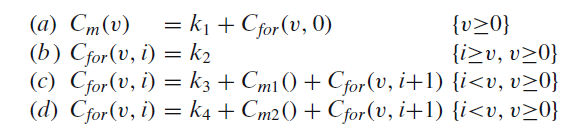
\includegraphics[width=0.6\textwidth]{basicExample.png}
    \caption{Relazioni di costo del programma \ref{lst:costAnalysisExample}}
\end{figure}

Dove $v$ indica la lunghezza dell'array $v$ e $i$ è la variabile di iterazione del ciclo, mentre $C_m,C_{m1},C_{m2}$ approssimano, rispettivamente il costo di esecuzione di $m$, $m_1$ e $m_2$.\\
I vincoli collegati ad ogni equazioni determinano le loro condizioni di applicabilità.\\
Ad esempio, l'equazione $(a)$ corrisponde al costo di esecuzione del metodo $m$ con un array di lunghezza maggiore di 0(indicato nella condizione $\{v > 0\}$), dove un costo $k_1$ è accumulato dal costo dell'esecuzione del ciclo, dato da $C_{for}$.
Le costanti $k_1,\dots,k_4$ sono valori differenti in base al modello di costo che viene selezionato.
Ovvero, se il modello di costo è basato sul numero di istruzioni eseguite, allora $k_1$ è 1 che corrisponde al costo dell'esecuzione di una istruzione java come \textit{int i= 0}.
Se il modello di costo si riferisce all'occupazione dell'heap, allora $k_1$ sarà 0, poichè l'istruzione precedente non alloca memoria.\\
Le equazioni $c$ e $d$ catturano rispettivamente il costo di esecuzione del branch \textit{then} e \textit{else}.
Si noti che, anche se il programma è deterministico, si tratta di equazioni non deterministiche che contengono le stesse condizioni di applicabilità. Ciò è dovuto al fatto che l'array v è astratto rispetto alla sua lunghezza e quindi i valori dei suoi elementi sono staticamente sconosciuti.\\
Alcuni aspetti interessanti dell'equazioni di costo:
\begin{itemize}
    \item Sono indipendenti dal linguaggio di programmazione
    \item Possono rappresentare diverse classi di complessità: lineare, quadratica, logaritmica, ecc.
    \item Possono essere utilizzate come abbiamo visto, per catturare una varietà di nozioni non banali di risorse: come il numero di chiamate a funzioni, il numero di allocazioni di memoria, il numero di accessi a memoria, ecc.
\end{itemize}
Un esempio già più completo che troviamo nel paper \textit{Automatic Inference of Upper Bounds for Recurrence Relations in Cost Analysis} \autocite{albert2008automatic}:
\begin{figure}[H]
    \centering
    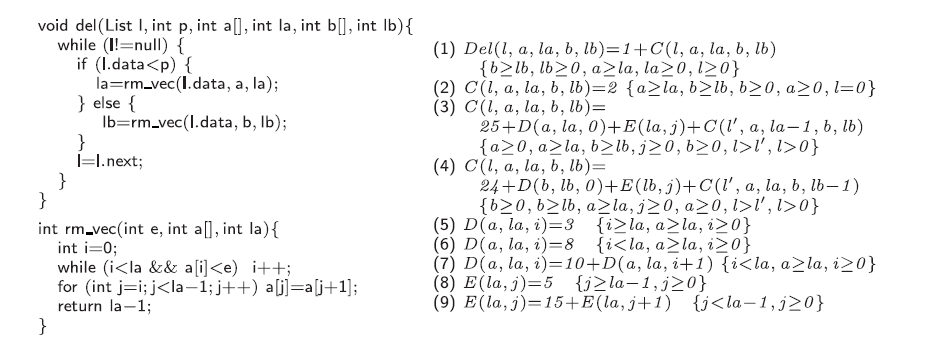
\includegraphics[width=0.9\textwidth]{costAnalysisExample.png}
    \caption{Esempio di Analisi di Costo}
    \label{fig:costAnalysisExample}
\end{figure}
Come possiamo vedere dall'immagine sopra, abbiamo a sinistra un programma scritto in java mentre a destra abbiamo l'analisi di costo del programma.\\
Il metodo $del$ prende in input una lista $l$, un pivot $p$, due array ordinati di interi $a$ e $b$ e $la$ e $lb$ che indicano rispettivamente le posizione occupate in $a$ e $b$.
Inoltre, si prevede che l'array $a$ contiene gli elementi inferiori al pivot $p$, mentre $b$ rispettivamente ne conterrà i valori maggiori o uguali.
Partiamo dal presupposto che tutti i valori in $l$ siano contenuti in $a$ o $b$, e il metodo $del$ rimuove tutti i valori in $l$ da $a$ o $b$ rispettivamente.
Il metodo $rm_{vec}$ rimuove un dato valore $e$ da un array $a$ di lunghezza $la$ e ne ritorna la nuova lunghezza.
Gli autori del paper \autocite{albert2008automatic},applicano l'analisi dei costi a questo programma, approssimando il costo del metodo $del$ in termini di istruzione bytecode eseguite.\\
La figura \ref{fig:costAnalysisExample} presenta i risultati dell'analisi, dopo aver effettuato una valutazione parziale.
Nei risultati dell'analisi le strutture dati vengono astratte in base alle loro dimensioni:$l$ rappresenta la lunghezza massima del percorso della corrispondente struttura dinamica, $a$ e $b$ sono le lunghezze degli array corrispondenti, mentre $la$ e $lb$ sono i valori interi delle variabili.
Ci sono nove equazioni che definiscono la relazione $ del $ che corrisponde al costo del metodo $del$ e 3 relazioni ricorsive ausiliarie C, D, E; ciascuna delle quale corrisponde a un ciclo:(C: Ciclo while in $del$, D: ciclo while in $rm_{vec}$ e E: Ciclo for in $rm_{vec}$).
Ogni equazioni è definita con una serie di vincoli che catturano le relazioni dimensionali tra i valori delle variabili della parte sinistra(lhs) e della parte destra(rhs).
Prendiamo in esempio le equazioni per $D$ Eq5. e Eq.6 rappresentano casi base per l'uscita dal ciclo ovvero quando $i \geq la$ e $a[i]\geq e$.
Per le nostre misurazioi di costo, vengono contati 3 istruzioni bytecode in Eq.5 e 8 in Eq.6.
Il costo per eseguire un iterazione del ciclo è rappresentato da Eq.7, dove la condizione $i < la$ deve essere soddisfatta e la variabili $i$ è incrementata di uno ad ogni chiamata ricorsiva.

\subsection{Relazione di Costo} 
Un'espressione di costo di base è un'espressione simbolica che indica le risorse accumulate e i blocchi fondamentali non ricorsivi per la definizione delle \textit{relazioni di costo}.
\newtheorem{definition}{Definizione}
\begin{definition}(Espressione di costo di base)\\
Le espressioni di costo sono della forma $$exp :: = a | nat(l) | exp + exp | exp * exp |exp^a |log _a (exp) | max(s) | \frac{exp}{a} | exp - a   $$
dove $a \geq 1$, $l$ è un'espressione lineare, $S$ è un insieme non vuoto di espressioni di costo, $nat : \mathbb{Z}  \rightarrow \mathbb{Q} ^+$ è definita come $nat(v) = max({v,0})$ e $exp$ soddisfa per qualsiasi assegnamento di $\overline{v}$ per vars($exp$) si ha $exp[ vars(\frac{exp}{\overline{v}})]$
\end{definition}

Le espressioni di costo di base godono di due proprietà:
\begin{itemize}
    \item Sono sempre valutate per valori non negativi
    \item Rimpiazzando una sottoespressione $nat(l)$ con $nat(l')$ tale che $l \geq l'$ , il risultato è un upper bound per l'espressione originale.
\end{itemize}
L'analisi dei costi di un programma produce multiple relazioni interconnesse, generando un \textit{sistema di relazioni di costo}(CRS)

\begin{definition}(Sistema di relazioni di costo)\\
    Un sistema di relazioni di costo S è un set di equazioni della forma $\langle C(\overline{x}) = exp + \sum_{i = 0}^n D_i(\overline{y_i}), \varphi \rangle$  dove $C$ e $D_{0,\dots, i}$ sono relazioni di costo; tutte le variabili in $\overline{x}$ e $\overline{y_i}$ sono variabili distinte, e $\varphi$ è una relazione di dimensione tra  $\overline{x} \cup vars(exp) \cup \overline{y_i}$.
\end{definition}

Dato $S$ sistema di relazioni di costo, $rel(S)$ indica l'insieme delle relazioni di costo definite in S, $def(S,C)$ indica il sottoinsieme di equazioni in S il cui lato sinistro è della forma $C(\overline{x})$.
Possiamo supporre che tutte le equazioni definite in $def(S,C)$ abbiano variabili con lo stesso nome nella parte sinistra.
Inoltre si suppone che ogni relazione di costo che appare nella parte sinistra dell'equazione $S$ deve essere in $rel(S)$.
\subsubsection{Semantica per CRS}
Data una CRS $S$, una call è della forma $C(\overline{v})$ dove $C \in rel(S)$ e $\overline{v}$ sono valori interi.
Le \textit{call} sono valutate in due fasi, in cui la prima permette la costruzione un albero di evoluzione, mentre la seconda ottiene un valore di $\mathbb{R}^+$ da aggiungere alla costante che appare nell'albero di valutazione.
Gli alberi di evoluzione sono costruiti espandendo iterativamente i nodi che includono chiamate alle relazioni. Ogni espansione avviene rispetto a un'istanza appropriata della parte destra di un'equazione applicabile. Se tutte le foglie dell'albero contengono un'espressione di costo di base, allora non ci sono più nodi da espandere e il processo termina. Questi alberi sono rappresentati utilizzando termini annidati, del tipo node(Call; Local\_Cost; Children), in cui Local\_Cost è una costante in $\mathbb{R}^+$ e Children è una sequenza di alberi di evoluzione.

\begin{definition}(\textbf{Albero di evoluzione})
    Data una CRS $S$, una call $C(\overline{v})$, un albero node $(C(\overline{v}); e; \overline{t})$ è un albero di evoluzione per $C(\overline{v})$ in S, indicato con $Tree (C(\overline{v},S))$, se:
    \begin{enumerate}
        \item c'è una denominazione parziale dell'equazione $\langle C(\overline{x}) = exp + \sum_{i = 0}^k D_i(\overline{y_i}), \varphi \rangle$
        \item esiste un assegnamento di valori interi $\overline{w}$ a $\overline{v_i}$ per $var(exp), \overline{y_i}$ rispettivamente tali che $\varphi[vars(exp)/\overline{w}, \overline{y_i}/\overline{v_i}]$ è soddisfacibile in $\mathbb{Z}$
        \item $e = exp[vars(exp)/\overline{w}]$, $T_i$ è un albero di evoluzione  $tree(D_i (\overline{v_i}, S))$ with $i \in 0,\dots,k$ 
    \end{enumerate}
\end{definition}

Nel processo di risoluzione di $C(\overline{v})$ ci possono essere diverse equazioni applicabili, e quindi diversi alberi di evoluzione.
Al passo 2 si cerca un assegnamento per le variabili nella parte destra di $\epsilon$. Al passo 3 gli assegnamenti sono applicati ad exp e si continua ricorsivamente valutando le call.
$Tree(C(\overline{v}, S))$ viene usato per denotare l'insieme di tutti gli alberi di evoluzione per $C(\overline{v})$.
\subsection{Stima del costo per Nodo}
Tutte le espressioni nei nodi sono istanze delle espressioni che compaiono nelle equazioni corrispondenti. Pertanto, il calcolo di $costr^+(\overline{x})$ e $costnr^+(\overline{x})$ può essere effettuato trovando innanzitutto un limite superiore di tali espressioni e quindi combinandoli attraverso un operatore di massimo. Prima calcoliamo gli invarianti per i valori che le variabili delle espressioni possono assumere rispetto ai valori iniziali e li utilizziamo per derivare limiti superiori per tali espressioni.\\
Calcolare le invarianti(in termini di vincoli lineari), in modo da raggruppare tutte le chiamate ai contesti di una relazione $C$, tra gli argomenti di una chiamata iniziale e ogni chiamata durante la valutazione che può essere fatta usando $Loops(C)$.\\
Ovvero, se è presente un vincolo lineare $\psi$ tra gli argomenti di una chiamata iniziale $C(\overline{x_0})$, quelli di una chiamata ricorsiva $C(\overline{x})$, indicato con $\langle C(\overline{x_0})\rightsquigarrow  (\overline{x}, \psi)\rangle$, e se esiste il ciclo $C(\overline{x_0}) \rightsquigarrow (\overline{y},\varphi)\in Loops(C)$ allora è possibile applicare il ciclo a uno o più step e prende un nuovo calling context $\langle C(\overline{x_0})  \rightsquigarrow (\overline{y}), \overline{\exists} \cup \overline{y_i}\dot \psi \land \varphi\rangle$.\\
Una volta che le invarianti sono state stabilite, è possibile determinare il limite superiore delle equazioni di costo massimizzando la loro parte nat indipendentemente. Questo approccio è reso possibile grazie alla proprietà di monotonia delle espressioni di costo. Considerando un'equazione di costo nella forma $\langle  C(\overline{x}) = exp + \sum_{i=0}^k C(\overline{y_i}), \varphi \rangle$ e un invariante $C(\overline{x_0})\rightsquigarrow C(\overline{x}, \varPsi) $ ,una funzione può calcolare un limite superiore $f'$ per ogni $f$ che compare nell'operatore $nat$. Tale funzione sostituisce $f$ con un limite superiore nelle espressioni $exp$ in cui non è possibile determinare un limite superiore e la funzione tornerà $\infty$. Se questa funzione è completa, ovvero se i $\varPsi$ e $\varphi$implicano che esiste un limite superiore per un dato $nat(f)$, allora possiamo trovare un limite superiore su $\varPsi '$.\autocite{amslaurea3135}
\newpage
\subsection{PUBS in pratica}
Prendiamo in considerazione il seguente esempio di programma dato in input a CostCompiler:
\begin{lstlisting}[language=Java,caption={Listing 1}]
struct Params {
	address: array[int],
	payload: any,
	sender: string
}
service PremiumService : (string) -> void;
service BasicService : (any) -> void;
(isPremiumUser: bool, par: any) => {
	if ( isPremiumUser ) {
		call PremiumService("pippo");
	} else {
		call BasicService( par);
	}
}
\end{lstlisting}

PUBS (Pratical Upper Bounds Solver) ha l'obiettivo di ottenere automaticamente un'upper bound in forma chiusa per i sistemi di equazioni di costo, calcola i limiti superiori per la relazione di costo indicata come "Entry", oltre che per tutte le altre relazioni di costo di cui tale "Entry" dipende.\\
Nell'output di PUBS vengono mostrati anche i passaggi intermedi eseguiti che coinvolgono il calcolo delle funzioni di classificazione e degli invarianti di ciclo.

\begin{figure}[H]
    \centering
    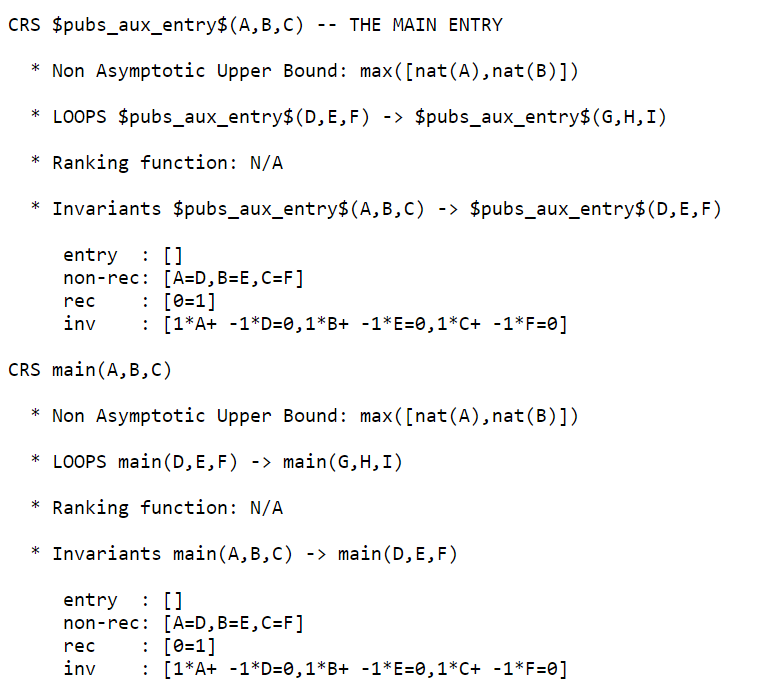
\includegraphics[width=0.9\textwidth]{pubs_example.png}
    \caption{Esempio di output PUBS su Listing 1}
\end{figure}
Come vediamo nell'immagine sopra, PUBS restituisce un analisi dell'intera equazione ($pub\_aux\_entry$) e delle singole funzioni da cui essa dipende, in questo caso $pubs\_aux\_if9$ e $pubs\_aux\_main$.\\
In questo caso con ``Listing1'' abbiamo un Upper Bound non Asintotico di $max(Nat(A), Nat(B))$ che ci determina che il costo del programma dipende dalle variabili A e B, e che il costo del programma sarà il massimo tra i due.\\
PUBS ha una grammatica che definisce l'equazione di costo che deve essere rispettata da ogni equazione di costo generata da CostCompiler, che è la seguente:
\newpage
\begin{lstlisting}[language=ANTLR, caption={Grammatica PUBS}]
<equation> ::= 
    eq(Head,costExpression,[listOfCall],[ListOfSizeRelation]).

<Head> ::= Name | Name(Par).

<costExpression> ::= nat(<variable>) 
            | <costExpression> + <costExpression> 
            | <costExpression> - <costExpression> 
            | <costExpression> * <costExpression> 
            | max(<costExpression>,<costExpression>).
                
<listOfCall> ::= [] | <call> <listOfCall>.
<call> ::= <function>(<listOfParameters>).
<listOfParameters> ::= [] | <variable> <listOfParameters>.
\end{lstlisting}
Dove $<$Head$>$ è il nome della entry che andremo ad analizzare insieme ai suoi parametri.
CostExpression è l'espressione di costo che rappresenta il costo della entry e rispetta la grammatica della aritmetica di Presburger.\\
ListOfCall è la lista delle chiamate alle altre entry, che sono rappresentate come $<$call$>$ e $<$listOfCall$>$, la lista di queste chiamate; in questo modo PUBS riesce a costruire un grafo delle dipendenze tra le entry.
Infine abbiamo $<$listOfSizeRelation$>$ che sarà la lista delle relazioni di costo che dipendono dalla entry che stiamo analizzando, e che PUBS andrà a calcolare.\\
Riportiamo un'altro esempio di equazione di costo generata da CostCompiler, questa volta per il programma scritto in Listing6:
\begin{lstlisting}[caption={Listing 6}, language=Java]
    service BasicService: (int) -> void;
    fn svc(i: int) -> void{
        for(m in (0,10)){
            call BasicService(i)
        }
    }
    (len : int) => {
        svc(len)
    }
\end{lstlisting}
Come vediamo, la funzione $init$ chiamerà la funzione $svc$ con parametro len, che a sua volta chiamerà la funzione BasicService per 10 volte, quindi il costo del programma sarà l'invocazione della funzione $svc + 10 \cdot nat(B)$, dove $nat(B)$ è l'invocazione del servizio \textit{BasicService}.\\
L'equazione di costo risultante sarà la seguente:
\begin{lstlisting}[language=Java,caption={Equazione di costo PUBS per Listing6}]
    eq(main(B),1,[svc(B)],[]).
    eq(svc(B),0,[for3(0, B)],[] ).
    eq(for3(M, B) ,nat(B),[for3(M+1, B)], [10>= M]).
    eq(for3(M, B) ,0,[],[M >= 10+ 1]).
\end{lstlisting}

Nella prima riga troviamo l'entry $main$ che prende in input B, con costo 1, chiama la funzione $svc$.
Quest'ultima andrà a chiamare la funzione $for3$ inserendo un'ulteriore parametro che sarà il counter del ciclo con parametro 0 e B, che avrà costo 0 in caso $M >= 10 + 1$ altrimenti avrà costo $nat(B)$.
E come controprova mostriamo ora il risultato di PUBS su Listing6:
\begin{figure}[H]
    \centering
    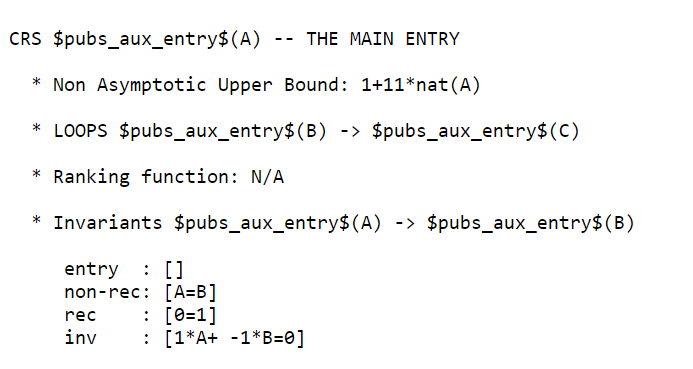
\includegraphics[width=0.9\textwidth]{pubs_example2.png}
    \caption{Esempio di output PUBS su Listing 6}
\end{figure}

\end{document}